% 1964 附加题（1）：矩形中的两圆构型（矢量重绘）
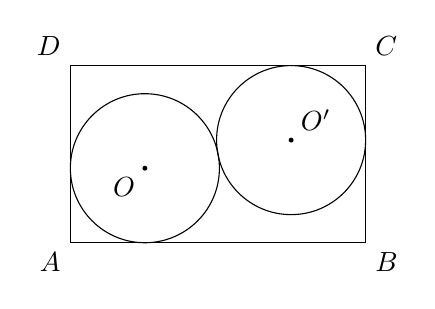
\begin{tikzpicture}[scale=0.75]
  \draw (0,0) rectangle (5,3);
  \node[below left] at (0,0) {$A$};
  \node[below right] at (5,0) {$B$};
  \node[above right] at (5,3) {$C$};
  \node[above left] at (0,3) {$D$};
  \draw (1.262,1.262) circle (1.262);
  \draw (3.738,1.738) circle (1.262);
  \fill (1.262,1.262) circle (1.2pt) node[below left] {$O$};
  \fill (3.738,1.738) circle (1.2pt) node[above right] {$O'$};
\end{tikzpicture}
